\chapter{Fundamentos de teledetección}

Esta clase tiene como objetivo familiarizarze con el entorno gráfico del \emph{Sentinel Aplication Toolbox (SNAP)}, un software de procesamiento de imágenes diseñado por la \emph{Agencia Espacial Europea (ESA)}, cuyas herramientas simplifican el trabajo con imágenes radar y ópticas.

Durante el curso se trabajará con imágenes de la región de triple frontera, que incluye el límite entre la provincia de Misiones en Argentina, Brasil y Paraguay. En esta zona (Figura \ref{fig:mapa}) se encuentra el Parque Nacional Iguazú (Argentina), el Parque Nacional Iguaçu (Brasil), el Aeropuerto Internacional Cataratas del Iguazú, los ríos Iguazú (frontera entre Argentina y Brasil) y Paraná (frontera entre Paraguay y Argentina), las ciudades de Foz de Iguaçu (Brasil), Ciudad del Este (Paraguay) y Puerto Iguazú (Argentina) y el embalse Ugugua-Í.

\begin{figure}[h!]
    \centering
    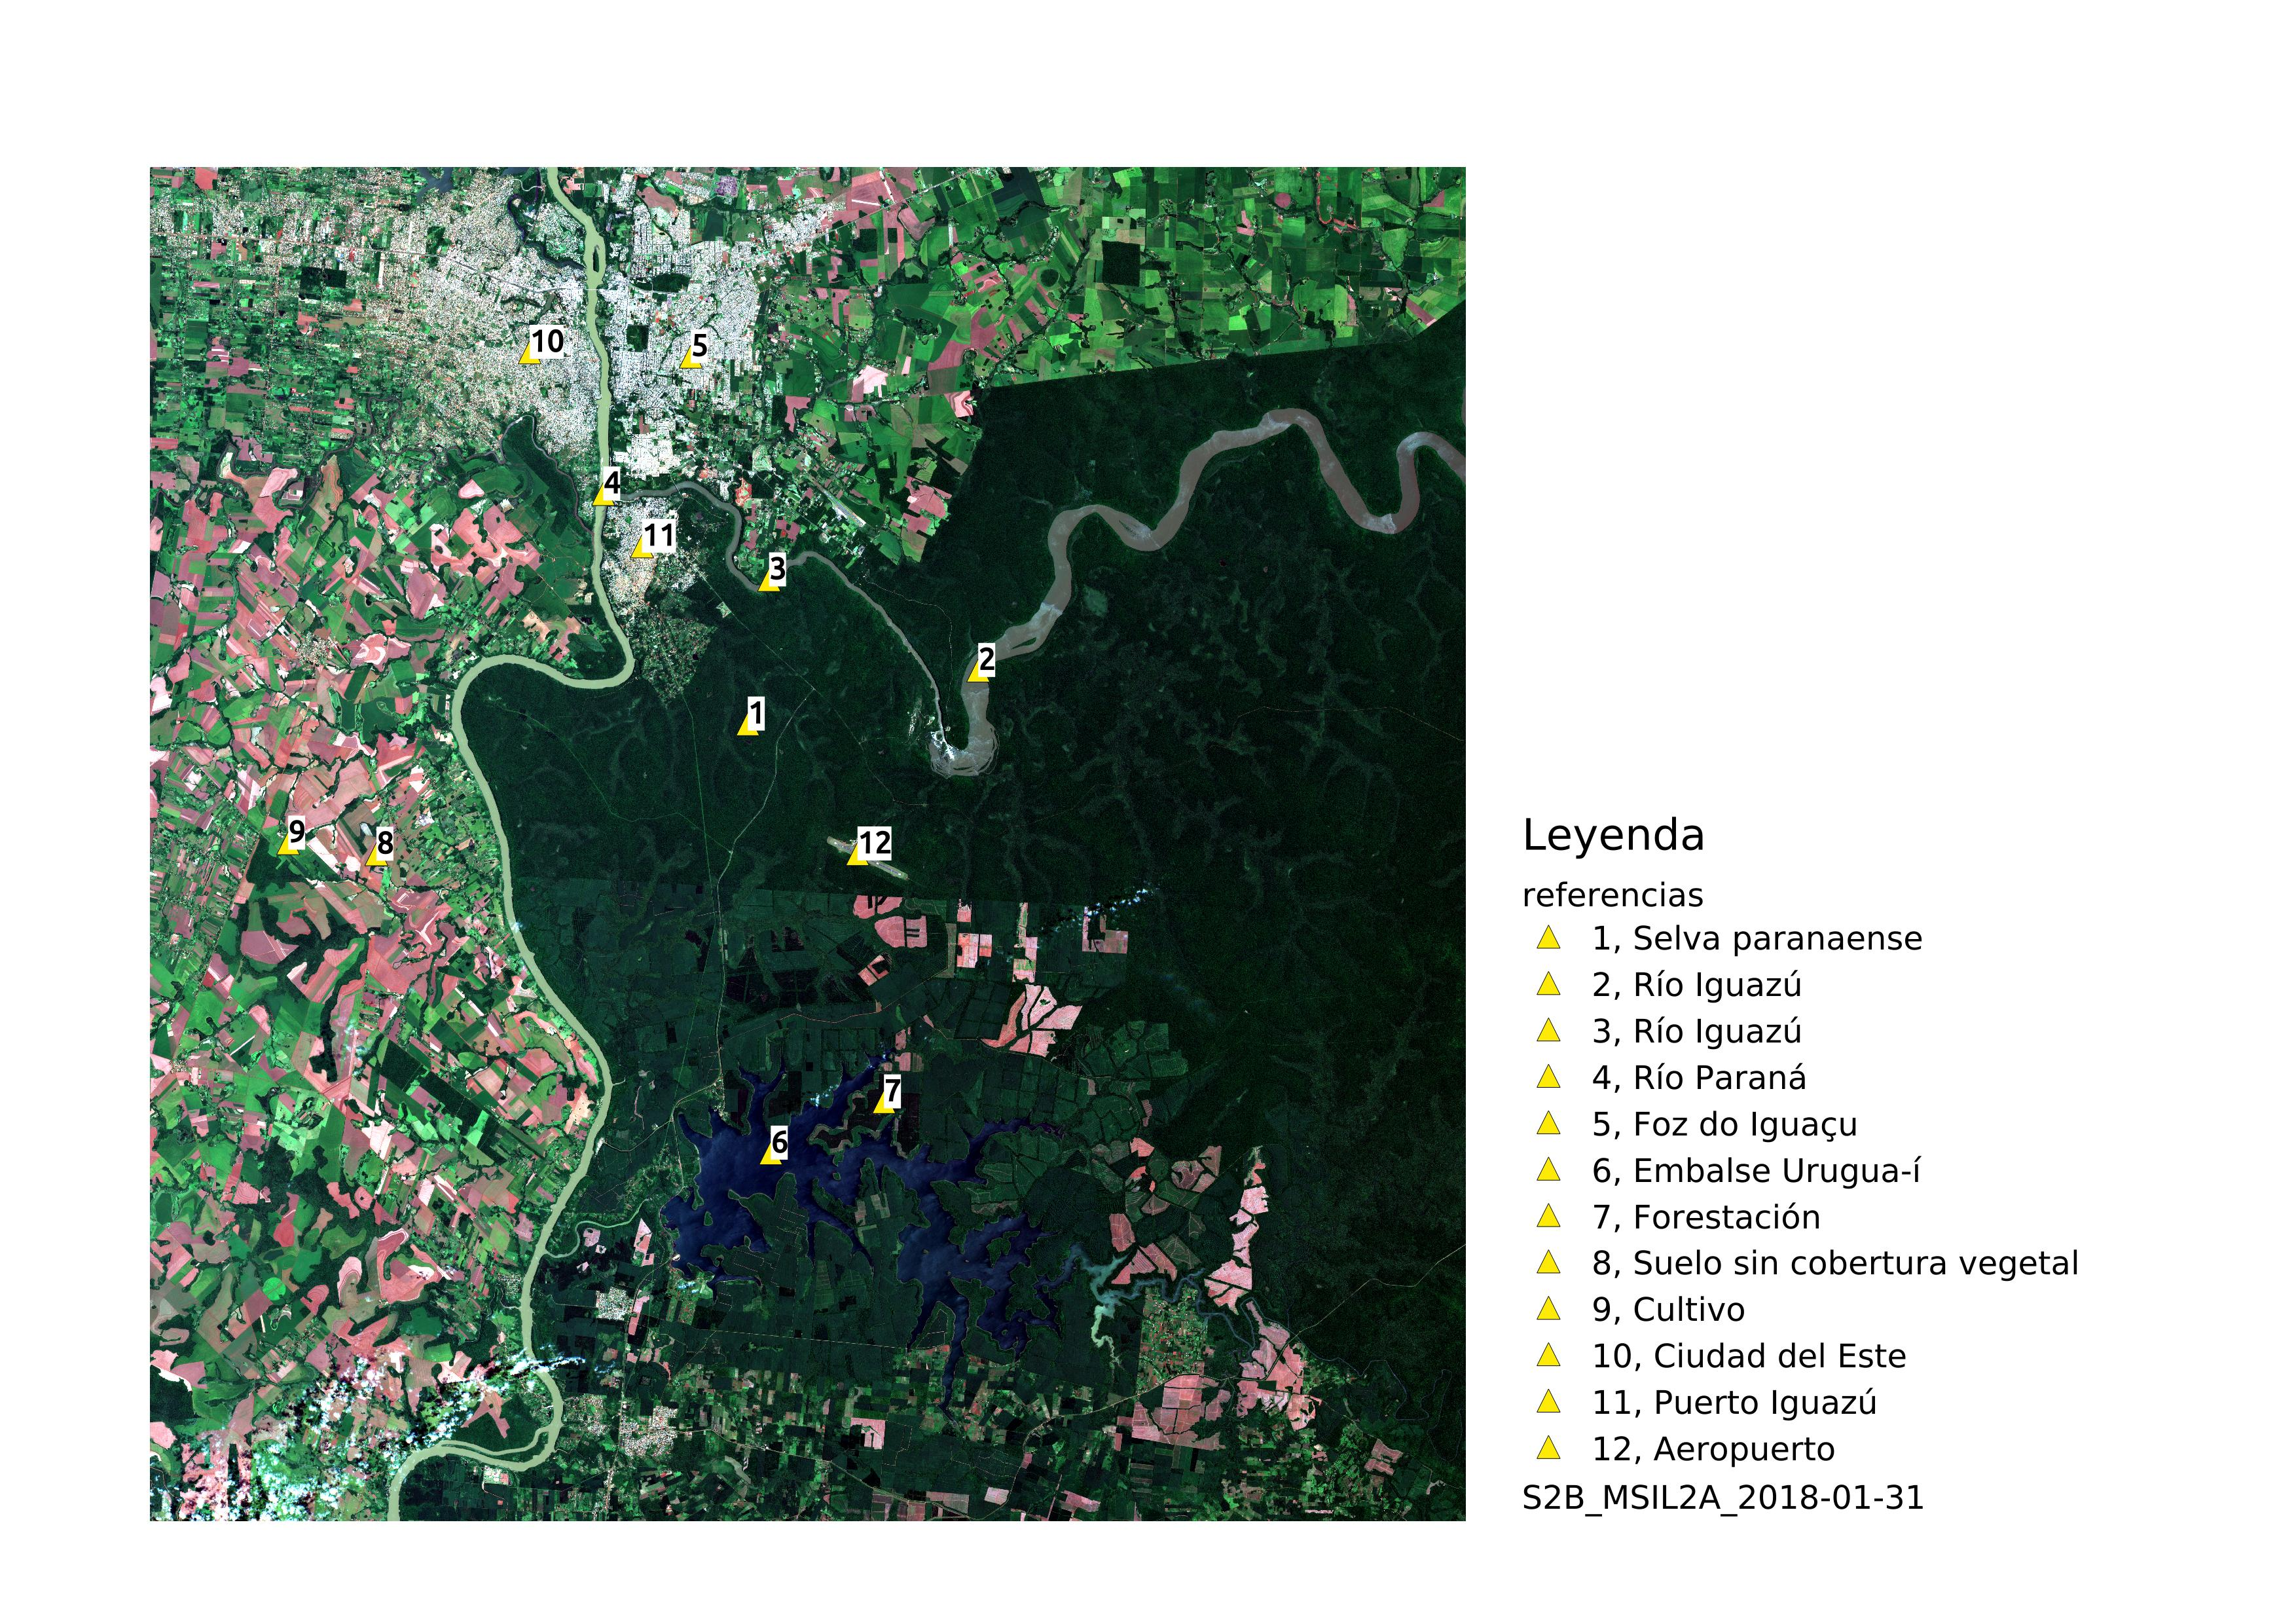
\includegraphics[width=0.7\textwidth]{fig:mapa.jpg}
    \caption{Mapa de la zona de triple frontera.}
    \label{fig:mapa}
\end{figure}

\section{Sobre esta guía}

A lo largo de la guía se utilizará como referencia la siguiente simbología:

\begin{itemize}
  \item \menu{Archivo>Abrir...} para indicar una ruta en el menú de un programa o una herramienta.
  \item \directory{Documentos/archivo.doc} para indicar una carpeta o archivo dentro de una carpeta.
  \item \texttt{Opción} para indicar una opción de configuración de un programa.
  \item \keys{ctrl + c} para indicar una combinación de teclas.
  \item \emph{SAR} para indicar un término específico o importante para la clase.
\end{itemize}

Las rutas estarán siempre definidas a partir de la carpeta \directory{material}.

\section{Interfaz gráfica del SNAP}

Descomprima el archivo \directory{material.zip}. Abra el programa SNAP, allí encontrará la interfaz gráfica del usuario (Figura \ref{fig:int})

\begin{figure}[h!]
    \centering
    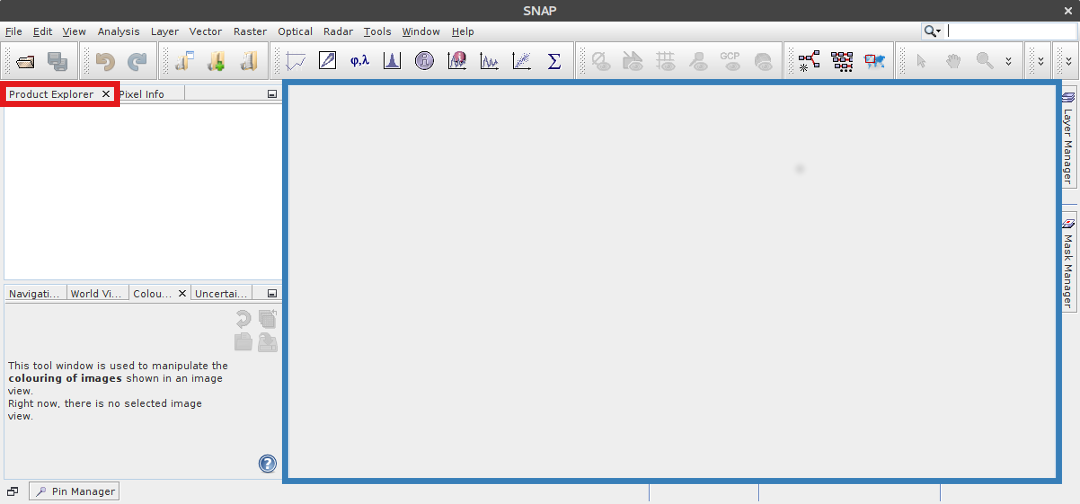
\includegraphics[width=0.6\textwidth]{fig:int.png}
    \caption{Interfaz gráfica del usuario. En recuadro azul muestra el área de visualización y el recuadro rojo al \menu{Product Explorer}.}
    \label{fig:int}
\end{figure}

\section{Apertura de imágenes}

Desde el menú \menu{File>Open product...} abra la imagen
\begin{center} \directory{LC08\_224-078\_2018-01-05.dim}.
\end{center}
Haga doble click sobre el nombre de la imágen y se desplegará, en el \menu{Product Explorer} un árbol que incluye:
\\
\dirtree{%
    .1 [1] LC08\_224-078\_2018-01-05.
    .2 Metadata.
    .2 Vector Data.
    .2 Bands.
}

En esta cobertura encontrará

\begin{itemize}
    \item \emph{[1] LC08\_224-078\_2018-01-05}: El número de elemento entre corchetes, indicando el orden en que se abrieron los productos y el nombre de la imagen.
    \item \emph{Metadata}: Los metadatos de la imagen y su historial de procesamiento.
    \item \emph{Vector Data}: Los vectores contenidos dentro de la imagen.
    \item \emph{Bands}: Las bandas de la imagen y las operaciones de álgebra entre bandas.
\end{itemize}

\section{Visualización}

Visualice la imagen en color real. Para ello, en el \menu{Product Explorer}, haga click derecho sobre el nombre de la imagen y seleccione \menu{Open RGB image windows}. En la ventana que se despliega podrá elegir las bandas (Figura \ref{fig:RGB}). Por defecto aparecerá la combinación que utiliza las bandas \emph{red}, \emph{green} y \emph{blue} de \emph{Landsat-8}. Para finalizar presione OK.

\begin{figure}[h!]
    \centering
    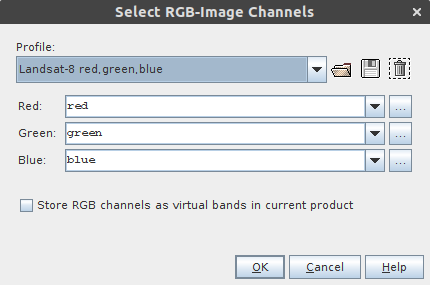
\includegraphics[scale=0.6]{fig:RGB.png}
    \caption{Ventana de combinación de bandas. Puede eligir una banda para cada canal del monitor (\emph{Red, Green, Blue}) o puede optar por una preseleccionada del menú \emph{Profile}}
    \label{fig:RGB}
\end{figure}

Explore la imagen con las herramientas de navegación y zoom (Figura \ref{fig:mono})

\begin{figure}[h!]
    \centering
    \subfloat[]{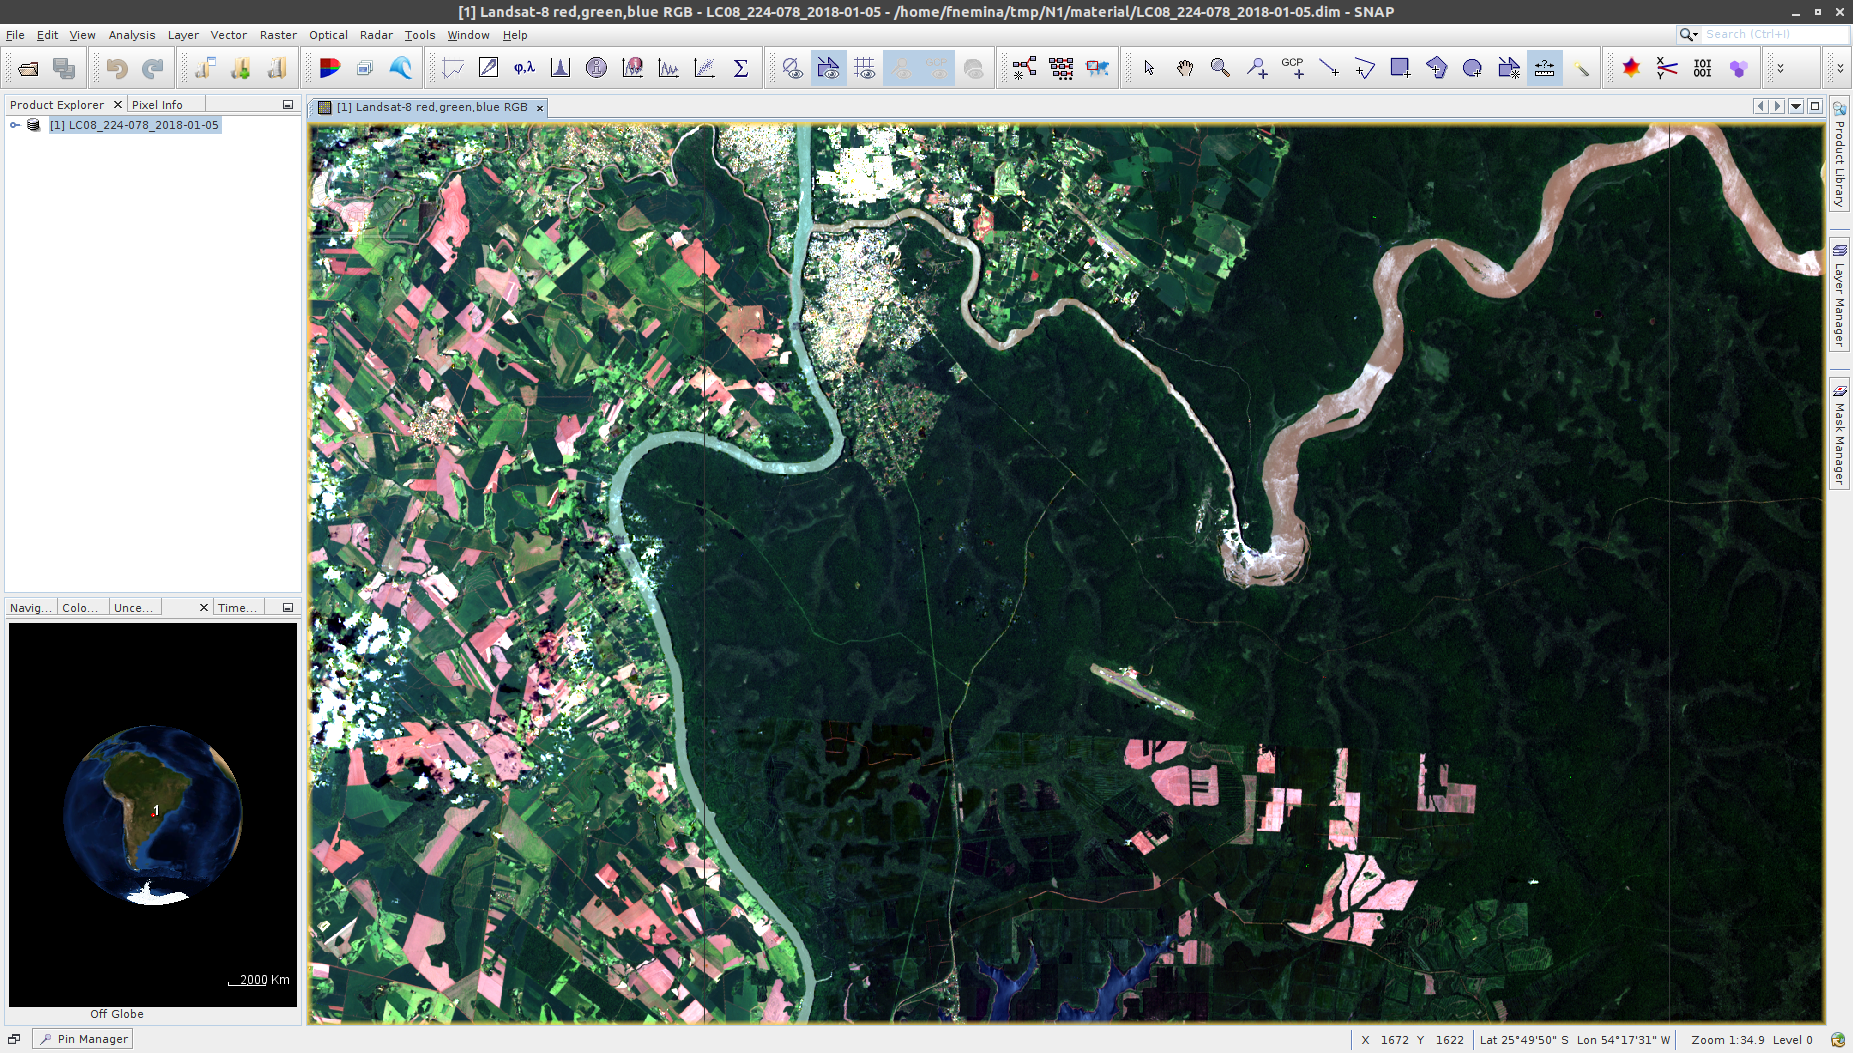
\includegraphics[width=0.6\textwidth]{fig:mono.png}}
    \\
    \subfloat[]{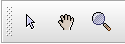
\includegraphics[scale=0.5]{fig:NAV.png}}
    \caption{(a) Imagen desplegada en el visualizador. (b) Herramientas de navegación. De izquierda a derecha: \menu{Selection tool}, para seleccionar objetos, \menu{Panning tool}, para moverse, y \menu{Zooming tool}, para hacer zoom.}
    \label{fig:mono}
\end{figure}

Localice dentro de la imagen el Aeropuerto Cataratas del Iguazú.

\section{Mediciones}

Para medir una distancia entre puntos se utiliza la herramienta \menu{Determines the distance between two points} (Figura \ref{fig:distancia} a) que se encuentra en la barra de herramientas.

\begin{figure}[h!]
    \centering
    \subfloat[]{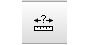
\includegraphics[scale=0.5]{fig:dico.png}}
    \\
    \subfloat[]{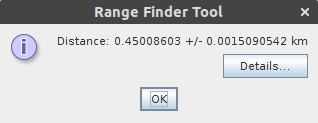
\includegraphics[width=0.3\textwidth]{fig:distancia.png}}
    \caption{(a). Herramienta de medición de distancia \menu{Determines the distance between two points}. (b) Ventana con el resultado de la medición.}
    \label{fig:distancia}
\end{figure}

Una vez seleccionado el icono, haga click derecho para trazar una linea entre los puntos a medir y finalice con doble click. El resultado y su incerteza (en Km), apareceran en una ventana emergente (Figura \ref{fig: distancia} b)Para utilizarla haga click sobre la herramienta y luego en un punto de la imagen para comenzar a medir.

Mida la longitud de la pista de aterrizaje del Aeropuerto Cataratas del Iguazú.

\section{Consulta de píxel}

Para obtener información sobre un pixel seleccione la pestaña \menu{Pixel info}, junto al \menu{Product explorer} (Figura \ref{fig:pixel}, y posiciónese sobre un pixel en la imagen.

\begin{figure}[h!]
    \centering
    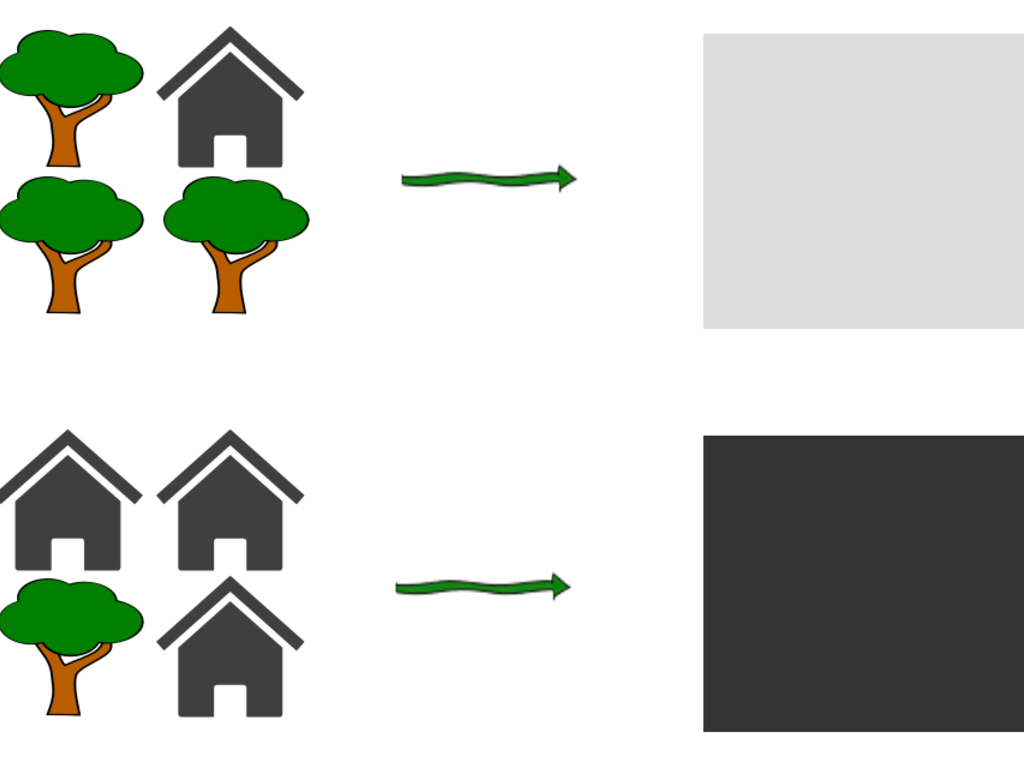
\includegraphics[width=0.3\textwidth]{fig:pixel.png}
    \caption{Herramienta de consulta de píxel. Puede verse la posición del píxel en la imagen, su latitud y longitud y el valor del píxel para la banda desplegada.}
    \label{fig:pixel}
\end{figure}

Allí encontrará la latitud y longitud, las coordenadas dentro del mapa y el valor del pixel en la banda abierta.

Halle las coordenadas en latitud y longitud Aeropuerto Cataratas del Iguazú.

\section{Multiples visualizadores}

Abra  y despliegue en color RGB las imágenes:
\begin{center} \directory{S2B\_MSIL2A\_2018-01-31.dim}.
\end{center}
y
\begin{center} \directory{MCD43A4.A2018039.h13v11.0065.dim}.
\end{center}

Ambas imágenes, junto con la anterior, corresponden a la misma zona y época del año.

Para ver las tres en simultáneo haga click en \menu{Window>Tile Horizontally}. Puede sincronizarlas con el botón \menu{Synchronises view across multiple image windows} (Figura \ref{fig:multiples}) y, al moverse o hacer zoom sobre una imagen, la acción se reproducirá en el resto, mostrándose las imágenes vinculadas. Para volver al modo habitual haga click en \menu{Window>Tile Single}. 

\begin{figure}[h!]
    \centering
    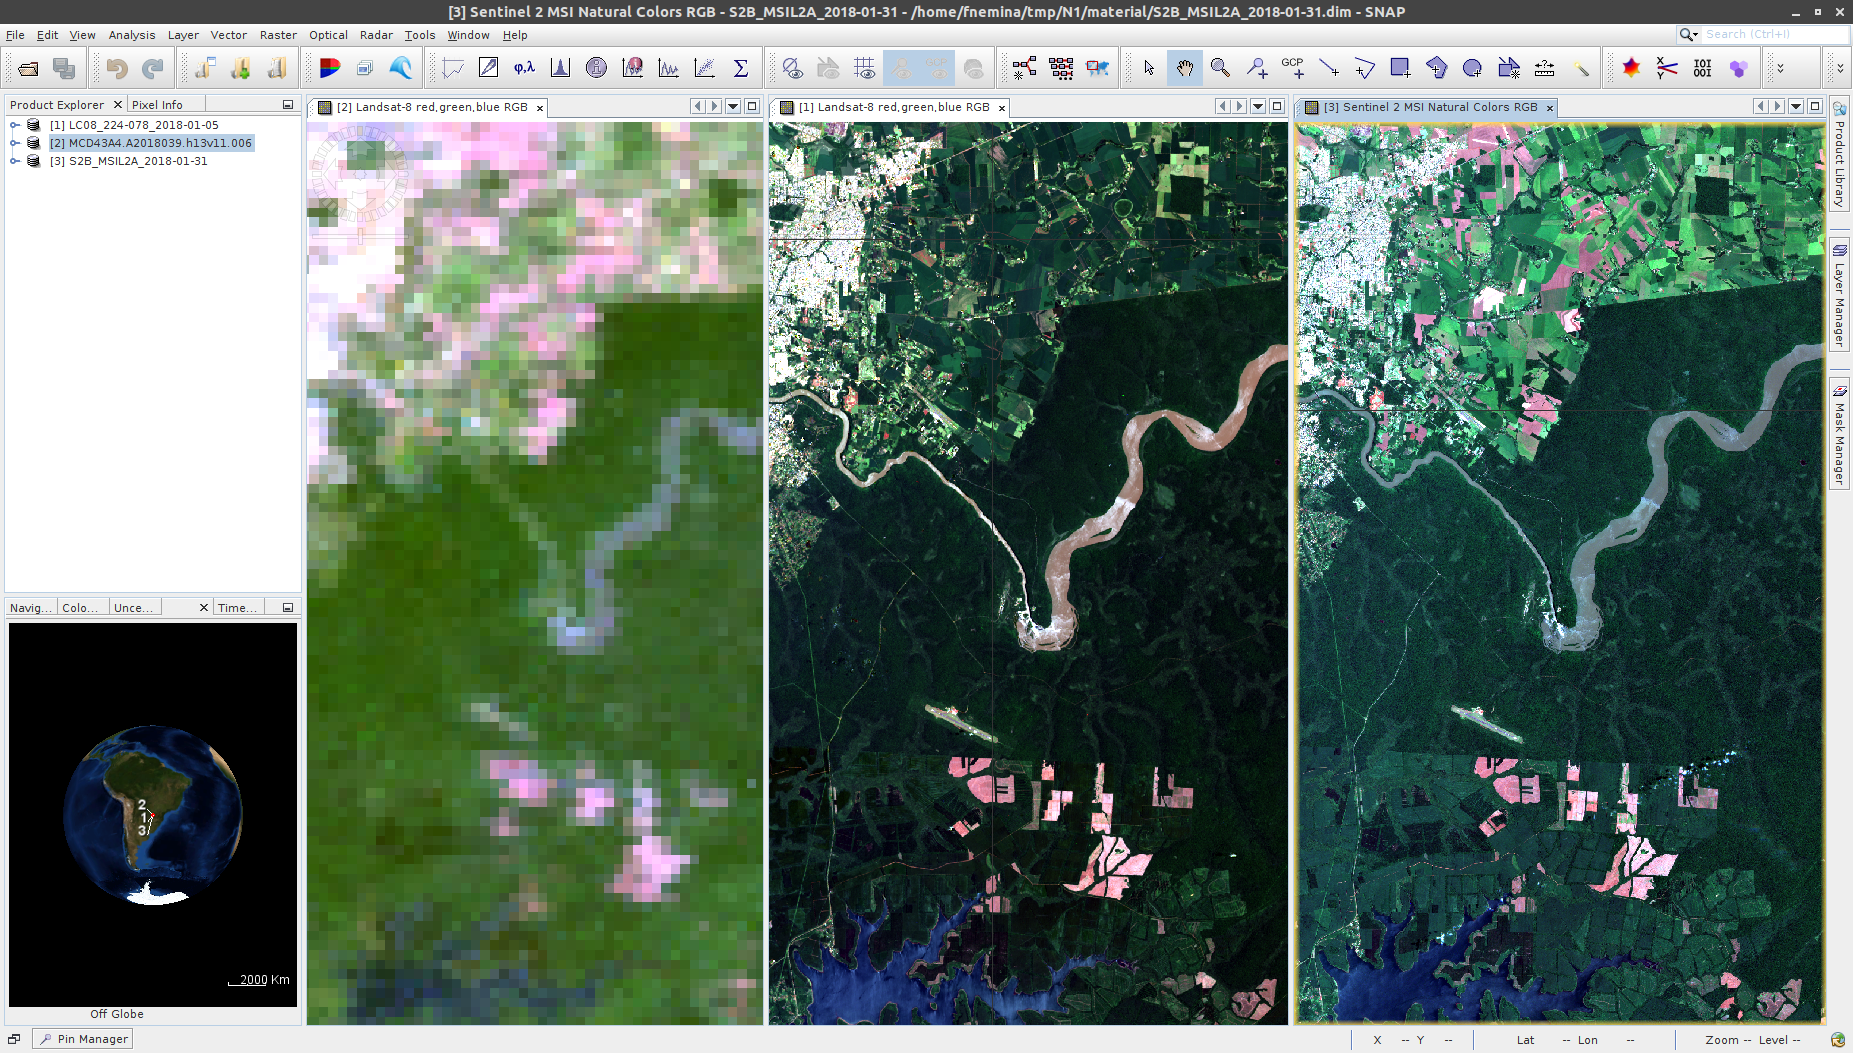
\includegraphics[width=0.6\textwidth]{fig:multiples.png}
    \caption{Múltiples visualizadores. Se destaca el botón \\ \menu{Synchronises view across multiple image windows}}
    \label{fig:multiples}
\end{figure}

\section{Actividad práctica}

\begin{enumerate}
  \item Con ayuda de la figura 1.1 identifique en la imagen los siguientes objetos:
  \begin{enumerate}
    \item El río Iguazú.
    \item El río Paraná.
    \item La ciudad de Puerto Iguazú.
    \item La zonas cultivadas al norte del río Iguazú con formas de parches en color verde.
    \item Las zonas cultivadas al oeste del río Paraná.
    \item La selva Paranaense.
    \item El embalse Urugua-í.
    \item La zona de forestaciones que rodea el embalse Urugua-í.
    \item El Aeropuerto Cataratas del Iguazú.
  \end{enumerate}

  \item Mida dentro de las tres imágenes los siguientes objetos:
  \begin{enumerate}
    \item El largo de la pista de aterrizaje del aeropuerto.
    \item El ancho del río Paraná frente a la ciudad de Puerto Iguazú.
    \item El perímetro de la ciudad de Puerto Iguazú.
    \item El perímetro del parche de selva Paranaense al norte del río Iguazú.
    \item El tamaño de un píxel.
  \end{enumerate}

  \item Identifique las coordenadas geográficas de los siguientes objetos:
  \begin{enumerate}
    \item El aeropuerto de las cataratas del Iguazú.
    \item La ciudad de Puerto Iguazú.
    \item La ciudad de Foz de Iguazú.
    \item Ciudad del Este.
    \item La desembocadura del embalse Urugua-Í.
    \item El cruce entre los ríos Paraná y Iguazú.
    \item Las cataratas del Iguazú donde el río Iguazú se angosta.
  \end{enumerate}
\end{enumerate}

Estas preguntas y actividades no serán evaluadas. Su objetivo es discutirlas en el foro de consultas e intercambio de la clase.
